
\section{Simulations}\label{sec-sim}
In this section we present a simulation study to assess the performance of our baseline test procedure from Section \ref{sec-model}. Before we proceed any fruther, we first need to specify some parameters that has an effect on the test statistic.

Our statistic $\widehat{\Psi}_T$ depends not only on the sample size $T$, but also on the choice of the kernel function $K(x)$ and the set $\mathcal{G}_T$. Throughout our numerical experiments, the Epanechnikov kernel $K(x) = \mathbbm{1}_{|x|\leq 1} \frac{3}{4} (1 - x^2)$ and the set $\mathcal{G}_T = \{(u, h): u = (5k)/T \text{ and } h = (3+5l)/T \text{ for some } k, l \in \mathbb{N}, k \le T/5, l \le T/20\}$ are used. The Epanechnikov kernel $K(x)$ and the set $\mathcal{G}_T$ with $|\mathcal{G}_T| = O(T^2)$ satisfy the conditions \ref{C-ker} and \ref{C-grid}-\ref{C-h} respectively.


\subsection{Size of the test}\label{subsec-sim-size}
We first provide some evidence on the size of the test. Data was generated by the model \ref{model1} under the null hypotheis $H_0: m=0$ with AR(1) errors
%\begin{equation}
%Y_t = m \Big( \frac{t}{T} \Big) + \varepsilon_t,
%\end{equation}
\begin{align*}
\varepsilon_t = a \varepsilon_{t-1} + \eta_t.
\end{align*}
Here $\eta_t$ are i.i.d. Gaussian inovations with $\mathbb{E}[\eta_t] = 0$ and $\mathbb{E}[\eta_t^2] = \sigma_{\eta}^2$. As was already stated before, such process satisfies the conditions \ref{C-err1} - \ref{C-err3}, therefore, \ref{theo-stat} holds true.

We choose parameters $a$ and $ \sigma_{\eta}^2$ such that the generated data resembles the real-life temperature dataset used for illustrating our method in Section \ref{sec-data}. In order to do that, we assume that the error structure in the real-life data also follows an AR(1) process and we estimate AR coefficient $a_1$ and the variance of the innovation $\sigma_{\eta}^2$ using the method described in Section \ref{subsec-error-var-ar}. We get the results $\hat{a}_1 = 0.5$ and $\hat{\sigma}_{\eta}^2 = 0.6$ which we use for generating errors $\{\varepsilon_t\}$.

Table \ref{tab:size_ll} shows size computations for various sample size ($T = 250, 350, 500, 1000$) and confidence levels ($\alpha = 0.01, 0.05, 0.10$). The simulations are based on 1000 replications and give results for one-sided tests under the null hypothesis $H_0: m=0$. As can be seen from the table \ref{tab:size_ll}, our test has approximately correct size even for small values of $T$ and the accuracy does not decrease with the sample size.
 
\begin{table}[H]
    \begin{center}
        \caption{Size of the test}
        \label{tab:size_ll}
        \centering
        % latex table generated in R 3.4.3 by xtable 1.8-2 package
% 
\begin{tabular}{rrrr}
  \hline
 & 0.01 & 0.05 & 0.1 \\ 
  \hline
250 & 0.007 & 0.033 & 0.072 \\ 
  350 & 0.005 & 0.041 & 0.087 \\ 
  500 & 0.015 & 0.054 & 0.078 \\ 
   \hline
\end{tabular}

    \end{center}
\end{table}

\subsection{Power of the test}\label{subsec-sim-power}

Tables \ref{tab:power_025_ll} - \ref{tab:power_075_ll} show power computations for various sample size ($T = 250, 350, 500, 1000$), confidence levels ($\alpha = 0.01, 0.05, 0.10$) and under different alternatives $H_1$. The simulations are based on 1000 replications and give results for one-sided tests under the alternative hypothesis $H_1: m \ne 0$. As can be seen from the tables \ref{tab:power_025_ll} - \ref{tab:power_075_ll}, our test has considerable power against fixed alternative even for small values of $T$. Furthermore, in accordance with the theory, the power of out test for a fixed significance livel $\alpha$ is an increasing function of the slope of trend. For a fixed slope of the trend, increasing the significance level also increases the power.


\begin{center}
Power of the test. Each table corresponds to different value of $a$, the endpoint of the trend function $m(\cdot)$.\\
\begin{minipage}{.45\textwidth}
\begin{table}[H]
    \begin{center}
        \caption{$a = 0.25$}
        \label{tab:power_025_ll}
        \centering
        % latex table generated in R 3.4.3 by xtable 1.8-2 package
% 
\begin{tabular}{rrrr}
  \hline
 & 0.01 & 0.05 & 0.1 \\ 
  \hline
250 & 0.032 & 0.092 & 0.155 \\ 
  350 & 0.018 & 0.090 & 0.199 \\ 
  500 & 0.069 & 0.169 & 0.212 \\ 
   \hline
\end{tabular}

    \end{center}
\end{table}

\end{minipage}
\begin{minipage}{.45\textwidth}

\begin{table}[H]
    \begin{center}
        \caption{$a = 0.50$}
        \label{tab:power_050_ll}
        \centering
        % latex table generated in R 3.4.3 by xtable 1.8-2 package
% 
\begin{tabular}{rrrr}
  \hline
 & 0.01 & 0.05 & 0.1 \\ 
  \hline
250 & 0.153 & 0.265 & 0.399 \\ 
  350 & 0.192 & 0.333 & 0.517 \\ 
  500 & 0.355 & 0.571 & 0.694 \\ 
   \hline
\end{tabular}

    \end{center}
\end{table}
\end{minipage}


\begin{minipage}{.45\textwidth}
\begin{table}[H]
    \begin{center}
        \caption{$a = 0.65$}
        \label{tab:power_065_ll}
        \centering
        % latex table generated in R 3.4.3 by xtable 1.8-2 package
% 
\begin{tabular}{rrrr}
  \hline
 & 0.01 & 0.05 & 0.1 \\ 
  \hline
250 & 0.321 & 0.471 & 0.590 \\ 
  350 & 0.416 & 0.620 & 0.744 \\ 
  500 & 0.686 & 0.846 & 0.900 \\ 
   \hline
\end{tabular}

    \end{center}
\end{table}
\end{minipage}
\begin{minipage}{.45\textwidth}
\begin{table}[H]
    \begin{center}
        \caption{$a = 0.75$}
        \label{tab:power_075_ll}
        \centering
        % latex table generated in R 3.4.3 by xtable 1.8-2 package
% 
\begin{tabular}{rrrr}
  \hline
 & 0.01 & 0.05 & 0.1 \\ 
  \hline
250 & 0.461 & 0.625 & 0.754 \\ 
  350 & 0.571 & 0.793 & 0.888 \\ 
  500 & 0.862 & 0.936 & 0.968 \\ 
   \hline
\end{tabular}

    \end{center}
\end{table}
\end{minipage}

\end{center}


\newpage
\section{Data analysis}\label{sec-data}
In this section, our methodology is applied to the problem of analyzing the temperature trends. For our analysis, we use climate data collected by The Met Office, a United Kingdom national weather service. The dataset of mean yearly temperature used to illustrate methodology from Section \ref{sec-model} consists of 359 observation of mean yearly temperature in England that covers years 1768 - 2017. The dataset of mean monthly temperature for various stations in the United Kingdom consists of 303 observations. 

\begin{figure}[ht!]
\centering
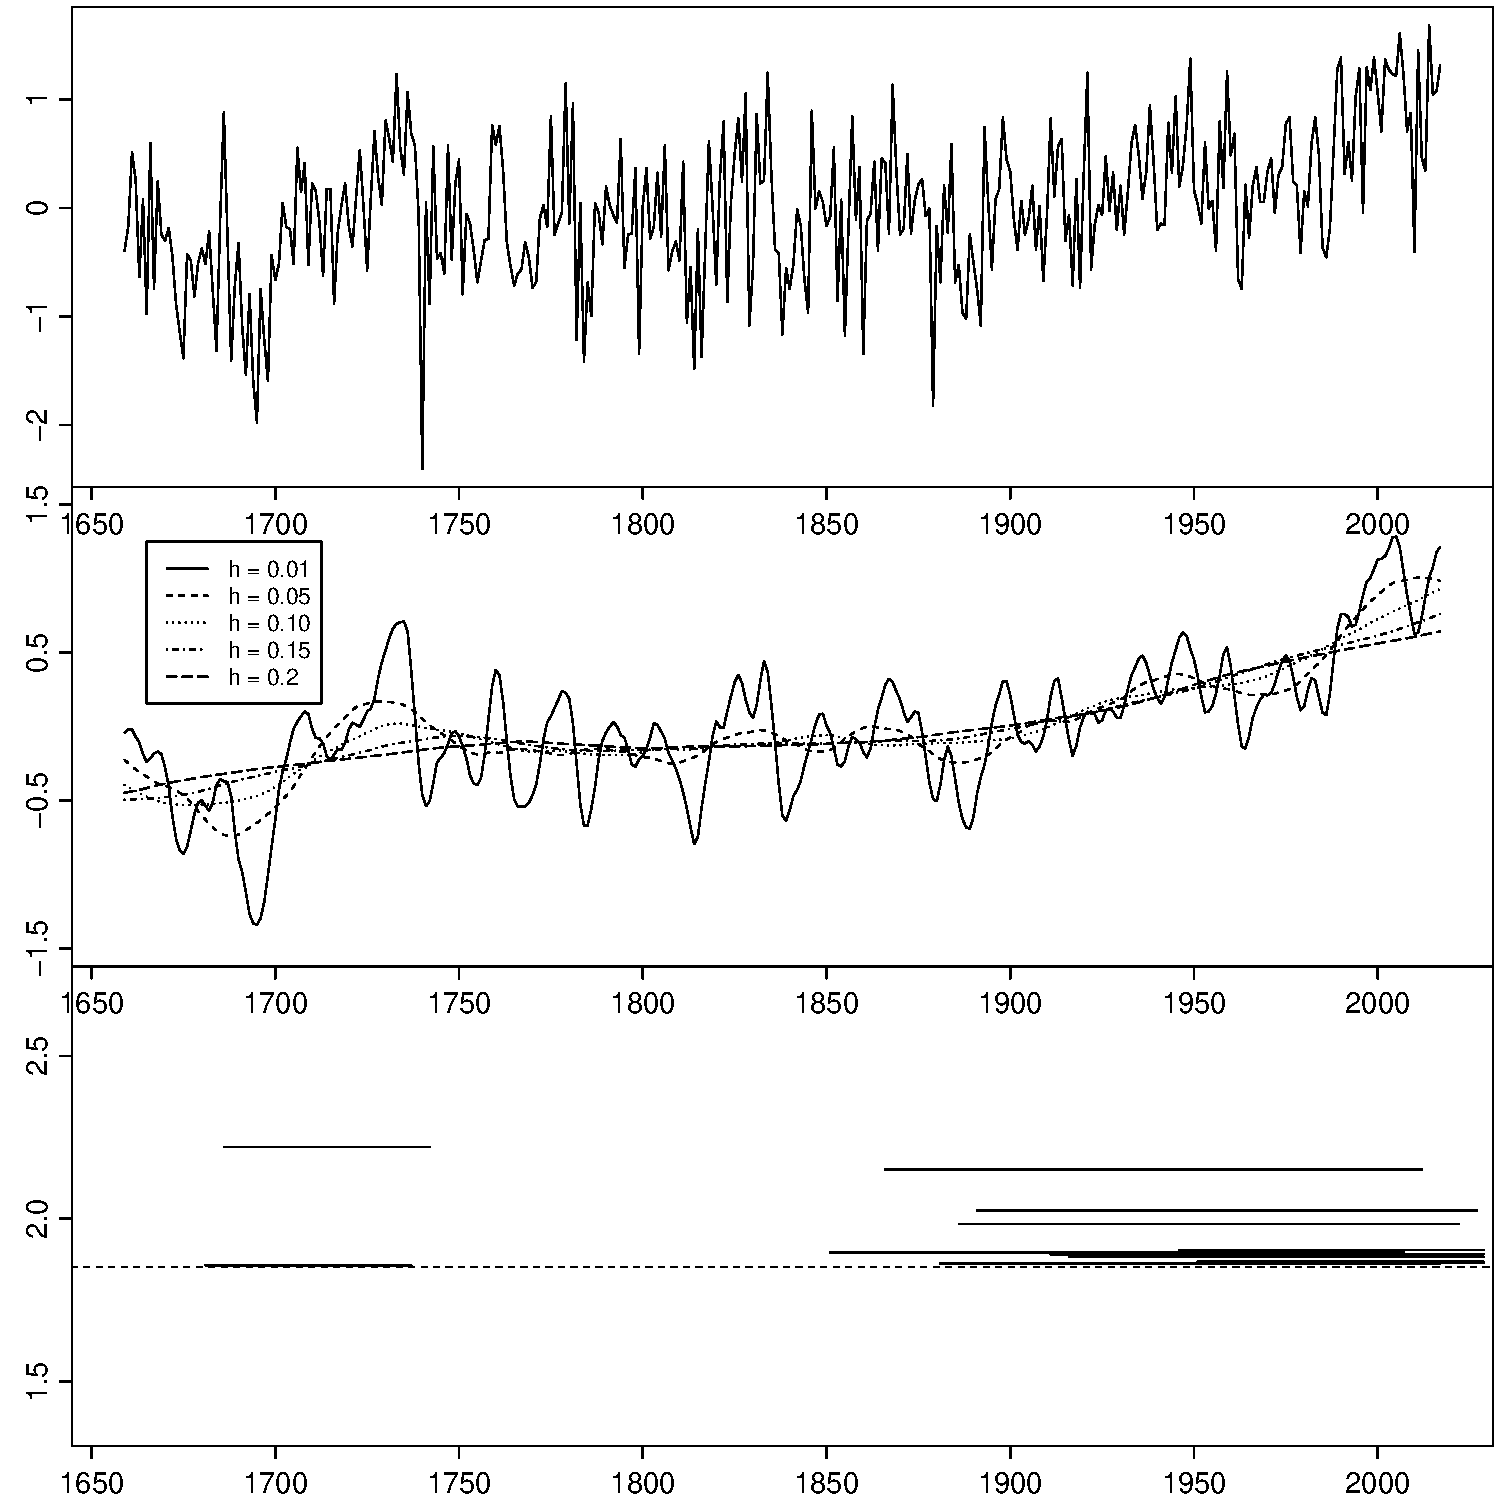
\includepdf[pages=-,pagecommand={},width=0.8\textwidth]{Coding/Output/threegraphics_testing_constant_method_ll.pdf}
\caption{Yearly temperature data for England\label{yearly_data}}
\end{figure}

